\documentclass[]{article}

\usepackage{graphicx}    % needed for including graphics e.g. EPS, PS
\usepackage{verbatim}   % used for multi line comments

\begin{document}         
\section{Introduction}
\label{introduction}
\input{styles/algorithm.sty}

Air traffic in the United States is predicted to increase significantly by the year 2025. The Next Generation Air Transportation System (NextGen) is the solution to capacity, safety, and efficiency problems that will result from this increase. The Federal Aviation Administration (FAA) is primarily responsible for the development of NextGen. The NextGen Concept of Operations identifies aircraft trajectory-based operations as a key capability required to ensure the success of NextGen. Four-dimensional (4-D) trajectory prediction algorithms predict an aircraft’s horizontal and vertical position at some time in the future and are used for conflict detection, metering, and other applications in air traffic management decision support tools (DSTs). Therefore, it is essential that the accuracy of trajectory prediction software be tested and validated. 

In previous work, the FAA has developed methodologies that identify trajectory prediction inaccuracies [Paglione et al., 2007] and have applied them in the accuracy testing of the User Request Evaluation Tool (URET) and En Route Automation Modernization (ERAM) [Paglione et al., 2001; Ryan et al., 2008]. Furthermore, as research and development (R\&D) advances for NextGen, the FAA is responsible for the development and validation of NextGen concepts. Therefore, the FAA has begun to develop an in-house developmental 4-D trajectory prediction infrastructure with the intent to mimic trajectory prediction capabilities during simulation and modeling activities in NextGen concept development. The FAA has studied the performance of these in-house tools [Ryan et al., 2008b; Santiago et al., 2010] which have been utilized in various research geared towards the improvement in the usability and accuracy of DSTs [Paglione et al., 2008; Paglione et al., 2010].

To support all these activities the FAA has developed a strong visualization tool infrastructure to investigate the accuracy of trajectories, and offer illustrations for the inaccuracies. This paper presents these tools as a visualization suite, and describes the process of evaluating trajectory modeling accuracy and performance. In addition, detail on how these types of investigations are developed, implemented, and presented is described. Two case studies are used to illustrate this process. The first case study focuses on the trajectory accuracy of two versions of ERAM during its acceptance testing. The second case study focuses on the accuracy performance of the in-house suite of trajectory predictors the FAA uses in NextGen concept development activities.

\section{Trajectory Modeling Tools}
\label{trajModelingTools}

Predicted trajectories are generated by a Decision Support Tool such as ERAM which utilize trajectory data in performing strategic planning. DSTs require an accurate and timely model of aircraft state and anticipated future path. The process by which trajectories are generated is known as a trajectory predictor or TP; the trajectory is the future four-dimensional path of the aircraft as measured in stereographic x-y coordinates, time and altitude. A TP predicts flight trajectories at a given time in the future based on initial conditions such as aircraft specific information (size, weight, engine type), velocity, horizontal position, altitude, environmental factors, other flights, and planned route. TP accuracy can be measured by post flight comparisons of the differences between predicted and observed aircraft trajectories using radar track recordings. As the predicted trajectory is the fundamental input that sustains the DSTs capabilities and functions, the accuracy of the TP has a direct impact on the DSTs overall performance and operational value.

\section{ERAM}
\label{ERAM}

The Lockheed Martin Corporation is developing En Route Automation Modernization (ERAM) as a new Air Traffic Control (ATC) system, which will replace URET and the existing Host Computer System (HCS) in the en route domain, for the Federal Aviation Administration. ERAM underwent a Formal Acceptance Testing (FAT) for Government Acceptance in 2007 in which it passed 93\% of over 4,000 requirements. Of those requirements eight were linked to the performance of ERAM’s TP and Conflict Probe for predicting potential separation violations in the en route domain. Of these eight accuracy requirements, ERAM passed only two of these eight requirements.[Ryan et al., 2008a]. Following the FAT, the contract developer and the FAA worked together in identifying problem reports (PRs). In time, the contract developer addressed critical PRs. Following the effort in resolving ERAM PRs, the system finally passed all eight accuracy requirements. The failed accuracy requirements included exceeding altitude error thresholds during flight descents and along track prediction deviations, which are scenarios to be investigated in the first case study. 

\section{Developmental Trajectory Predictors}
\label{devTP}

 In the R\&D involved in the development of Trajectory-based Operations (TBO) NextGen validation concepts, simulation and modeling activities are performed. Simulation and modeling (S\&M) aids the FAA investigate and evaluate the impact new concepts on air traffic. Due to the nature of S\&M work, it is expensive and often infeasible to integrate an operational system (e.g. ERAM) into the R\&D environment. In addition, it may be the case that modeling work involves a modification or enhancement to a system, in order to evaluate the system, thus simulation of the system is needed. The FAA has designed and implemented an infrastructure of several developmental trajectory predictors, each of which are described below.
Linear Predictor – The simplest of the predictors, models flights in a straight line from current direction and speed.
Flight Plan – Models aircraft according to flight plan.
Hybrid Merge – Models according to flight plan, if aircraft deviates from the plan it will switch to a linear prediction.
Basic Aircraft Data (BADA) – Extends the Hybrid Merge predictor to include changes to aircraft speed and altitude (aircraft performance).

\subsection{Development Background}
\label{devBackground}

The Simulation and Analysis (S\&A) Team, AJP-661, has been involved in testing and evaluation of DSTs and concept development work for improvement to DSTs, specifically trajectory predictors and conflict probe tools, for years. The S\&A Team has measured the conflict prediction accuracy of URET [Cale et al. 1999], and the trajectory modeling accuracy of both URET and CTAS [Cale et al. 1999 and Paglione et al. 1999], and the trajectory and conflict prediction accuracy of ERAM [Ryan et al., 2008a]. Furthermore, the S\&A Team is currently involved in the development of trajectory and conflict prediction algorithmic improvements for ERAM Post Release 3, under the NextGen Separation Management: Modern Procedures project.

In support of all the activities S\&A Team has been involved with, a partnership was formed with the Software Engineering, Graphics and Visualization (SEGV) research group at Rowan University. Through this collaboration SEGV has developed visualization tools to aid the analysts investigating trajectory modeling data of DSTs. One major activity this collaboration supported was the aforementioned ERAM formal acceptance testing [Rusu et al., 2009b]. This set of visualization tools has been transformed into a tool suite, Trajectory Analysis Graphical Suite (TAGS), which is actively developed and maintained today. Three of the tools focusing on trajectory prediction accuracy will be the focus of our case studies [Rusu et al., 2007].

\section{Trajectory Analysis Graphical Suite}
\label{trajAnalysisGraphicalSuite}

The Trajectory Analysis Graphical Suite is a collection of visualization tools that aid FAA analysts in the evaluation of trajectory predictor accuracy data. The novelty exists in the suites ability to package trajectory accuracy results using a graphical user interface, which helps analysts illustrate reasons for inaccuracies.

\subsection{Trajectory Galaxy Visualization 3D}
\label{trajGalaxyVis3d}

\subsection{Star Glyph}
\label{starGlyph}
A star glyph is a multivariate graphing technique in which each variable represents a ray, or "spoke," each of which extends out via a connecting line from a common origin with equal angular distance between each spoke. The length of each line is proportional to the magnitude of the variable compared to the maximum value of all the variables citation2. Star glyphs are extremely effective at locating outliers and determining where data begins to cluster.

\subsection{Basic Star Glyph}
\label{basicStarGlyph}
A basic star glyph, with six rays extending out from the origin in equal angular distances, is presented in Figure \ref{fig:basicGlyph}. A star glyph has two dimensions: a quantifiable dimension and a categorical dimension. The quantifiable dimension is a single value and the magnitude of this value is represented by the length of a spoke. The quantifiable value is grouped by categorical data. For instance, the star glyph in Figure 1 represents the average amount of food a dog in a particular kennel will consume daily. The data is grouped by the breed of the dog (e.g. s4 represents all beagles, while s2 represents all St. Bernards). We can easily see that, on average, a St. Bernard will consume much more food than all other types of dogs, while a beagle will consume close to the least amount of food. This graph allows us to recognize an outlier (e.g for exclusion or further analysis).

\begin{figure}[htb]
\begin{center}
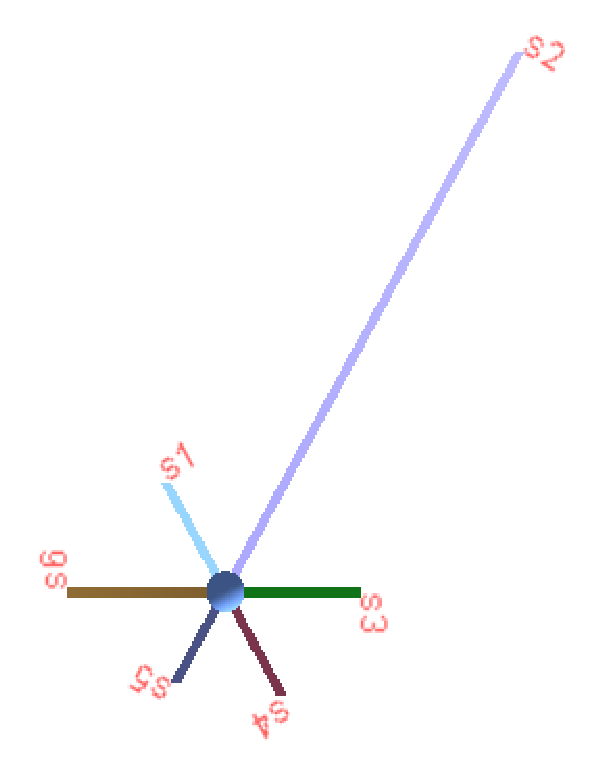
\includegraphics[width=0.4\textwidth, keepaspectratio=true]{images/basicStarGlyph}
\end{center}
\caption{A Basic Star Glyph}
\label {fig:basicGlyph}
\end{figure}

\subsection{An Additional Attribute}
\label{ss:additional_attribute}

TrajGalaxyViz3D has the option of adding another attribute to compare more data. This attribute can be any arbitrary value represented in the form of sphere where the radius of the sphere is proportional to the attribute's value.

Consider the graph in Figure \ref{fig:spheres} representing the average number of miles per day an athlete runs grouped by the sport he plays.  Let the size of the sphere represent the average weight of the athletes.  Now, assume that the large green sphere to the bottom right represents American football players while the bottom purple sphere represents cross country runners.  We can see that the cross country runners, on average, run much longer than football players, however, football players are generally much heavier.

The addition of the sphere allows for more data to be added to the graph without becoming overwhelming. Furthermore, the color of the spheres can put the data in a particular category. For example, in Figure~\ref{fig:spheres} the two blue spheres on top and top-right represent lacrosse players. The sphere at the top represents lacrosse players in the fall, whereas the sphere on the top-right represents lacrosse players in the spring. From this graph we can see that lacrosse players run more in the spring since they are presumably better trained by that time. Table \ref{table:sports} shows what a sample data set for the previous graph might look like.

\begin{figure}[htb]
\begin{center}
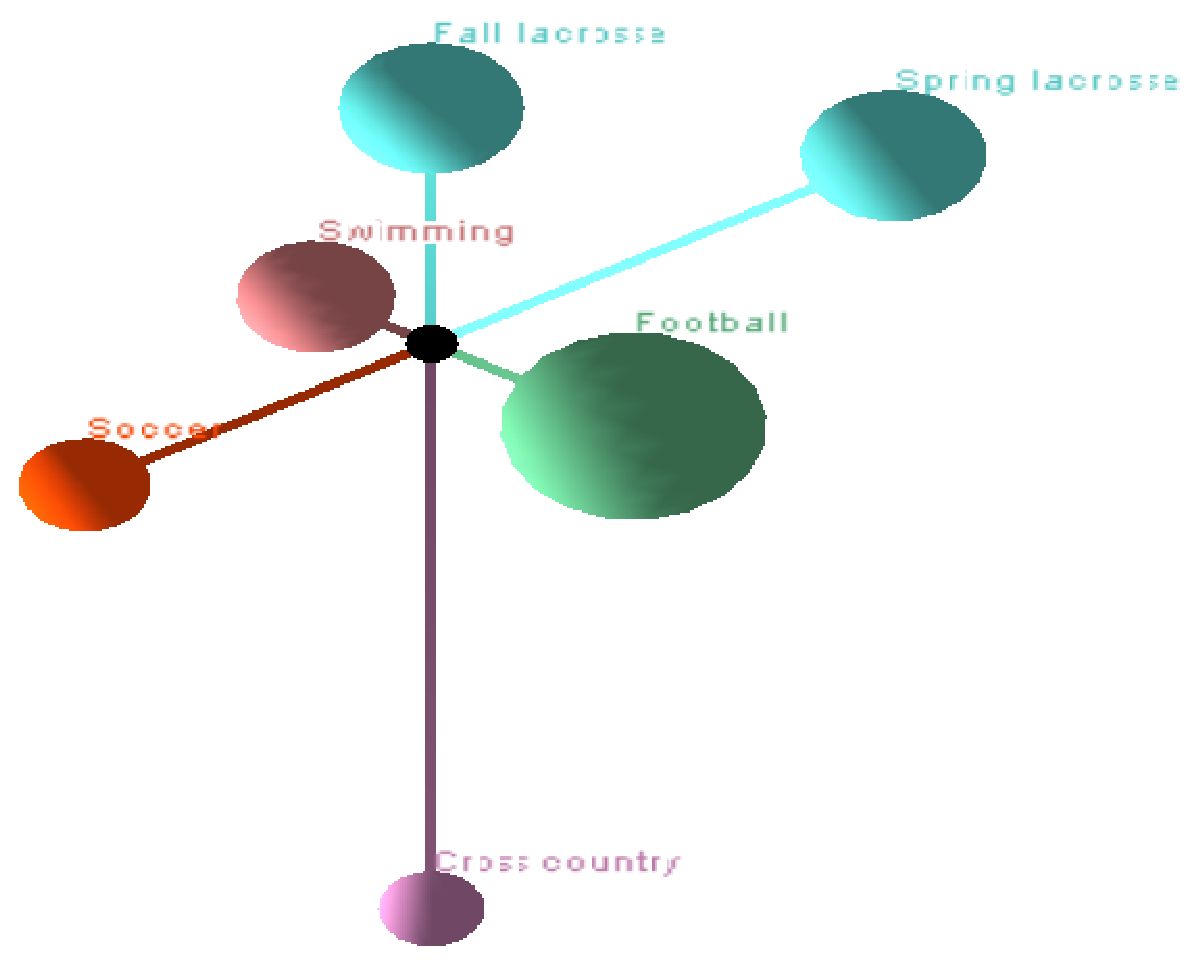
\includegraphics[width=0.6\textwidth, keepaspectratio=true]{images/starsphere}
\end{center}
\caption{A Star Glyph with Spheres}
\label {fig:spheres}
\end{figure}

\begin{table}
\begin{center}

    \begin{tabular}{ | c | c | c | c |} \hline
    \textbf{Sport}      & \textbf{Miles}    & \textbf{Weight}   & \textbf{Color}    \\ \hline
    American football   & 1.5               & 250               & Green             \\ \hline
    Cross country       & 8                 & 130               & Purple            \\ \hline
    American soccer     & 4                 & 160               & Red               \\ \hline
    Swimming            & 0.5               & 140               & Orange            \\ \hline
    Fall lacrosse       & 3                 & 150               & Blue              \\ \hline
    Spring lacrosse     & 5                 & 150               & Blue              \\ \hline
    \end{tabular}
    
\end{center}
\caption{Tabular data for sports star glyph}
\label {table:sports}
\end{table}

\subsection{An Additional Attribute}
\label{ss:additional_attribute}

\subsection{Clustered Mean Graph}
\label{ss:clustered}

The addition of spheres to the visualization increases the clutter of a graph.  This creates a cluster graph as shown in Figure~\ref{fig:clustered}, making it difficult to analyze the groups inside the cluster, but easily identifying and analyzing the outliers of the graph. A disadvantage to the traditional star glyph visualization is that effectiveness decreases signficiantly for cluttered data sets @todo citation needed. In order to mitigate the clutter, TrajGalaxyViz3D provides an option of graphing a clustered mean star glyph.

Wherever data is closely similar, the visualization clusters that data into a "blob" of spheres. It removes the labels for clustered data and leaves the labels for the outliers.

The average data are always clustered in the center and the outliers extend out in a position that represents their absolute value from the average cluster.

\begin{figure}[htb]
\begin{center}
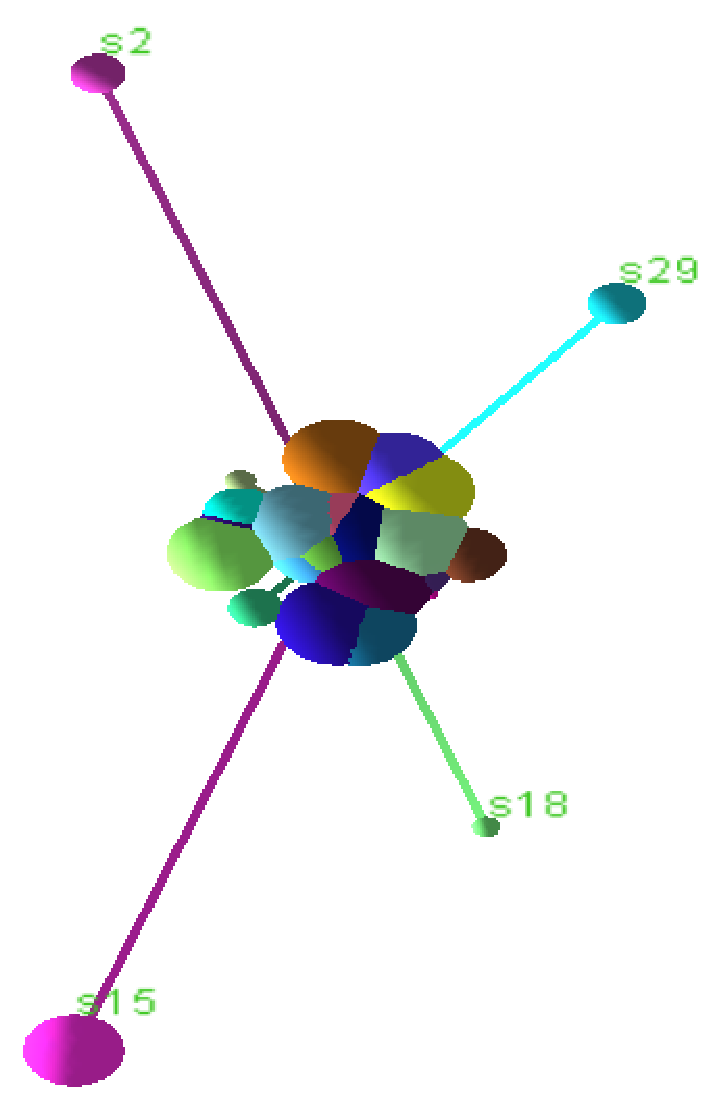
\includegraphics[width=0.4\textwidth, keepaspectratio=true]{images/clustered}
\end{center}
\caption{A Star Glyph with Spheres}
\label {fig:clustered}
\end{figure}

We use the following algorithm to determine whether or not data should be included in the cluster.

\begin{Algorithm} {Clustering} {\sf
\vspace*{10pt}
\row {\em Input:} The data points of the nodes.
\row {\em Output:} A graph with nodes. Nodes in the graph are clustered if they are close to the average of the data points. Nodes that are not clustered are the outliers and their positions are the absolute values from the average of the nodes.
\vspace*{10pt}

\row  \cforeach\ $node$ in $nodes$
\begin{nested}
    calculate $avg$ for all nodes
\end{nested}
\row  \cforeach\ $node$ in $nodes$
\begin{nested}
\row \cif\ $node$ is close to $avg$
\begin{nested}
\row add $node$ to cluster
\end{nested}
\end{nested}

}
\end{Algorithm}
\\

Clustering data is increasingly more important in analysis especially in a top such as data mining. By abstracting the details of the average, an analyst can focus only on the outliers. In data mining, an outlier could be a group of people that has not been marketed to or fraudlent data in a company's budget.

\subsection{Comparison of Multiple Star Glyphs}
\label{ss:comparison}

Finally, we add the last dimension of our visualization.  A single star glyph exists on a single two dimensional plane, therefore, since this is a three dimensional graph, we have the third dimension to display multiple star glyphs.  This allows us to compare several results to each other.

For instance, consider that Figure \ref{fig:multiple} represents surveys taken by several different news agencies on which of six different companies produces the best ice cream.  The distance of the spokes represents the average score of the ice cream producer (from 0 to 5, 5 being best), while the size of the sphere represents the amount of sales that producer had last year.  Each separate glyph represents a separate survey.  By displaying the three different surveys in same visualization, we can determine, among other things, which survey was more biased toward a particular producer.

\begin{figure}[htb]
\begin{center}
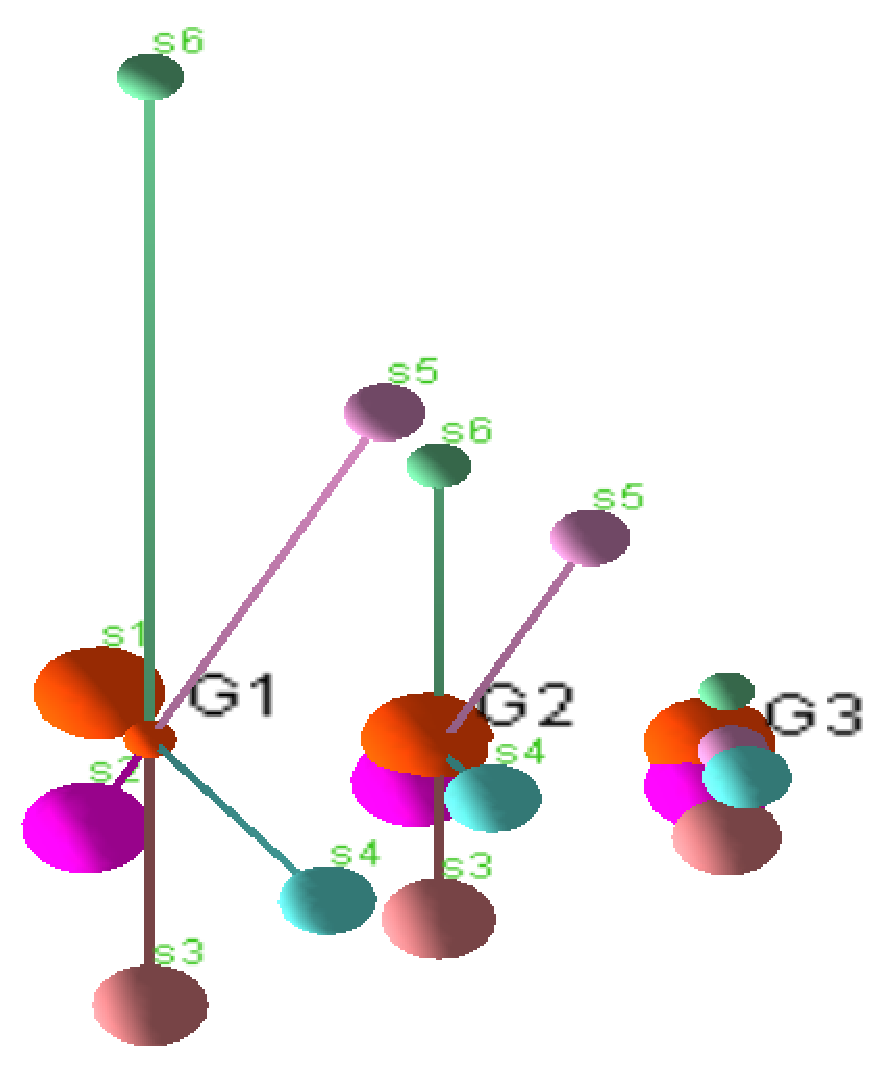
\includegraphics[width=0.4\textwidth, keepaspectratio=true]{images/multiple}
\end{center}
\caption{A Star Glyph with Spheres}
\label {fig:multiple}
\end{figure}

\subsection{User Interaction}
\label{ss:user_interaction}

Allowing the user to easily navigate the scene to focus on points of interest would give him invaluable insight into the information presented.  One basic interaction is the ability to rotate the star glyphs in any direction, allowing the user to get the perspective he desires (see Figure~\ref{fig:angle}), and to move about the visualization to find the exact camera position required for analysis of a focal point.

\begin{figure}[htb]
\begin{center}
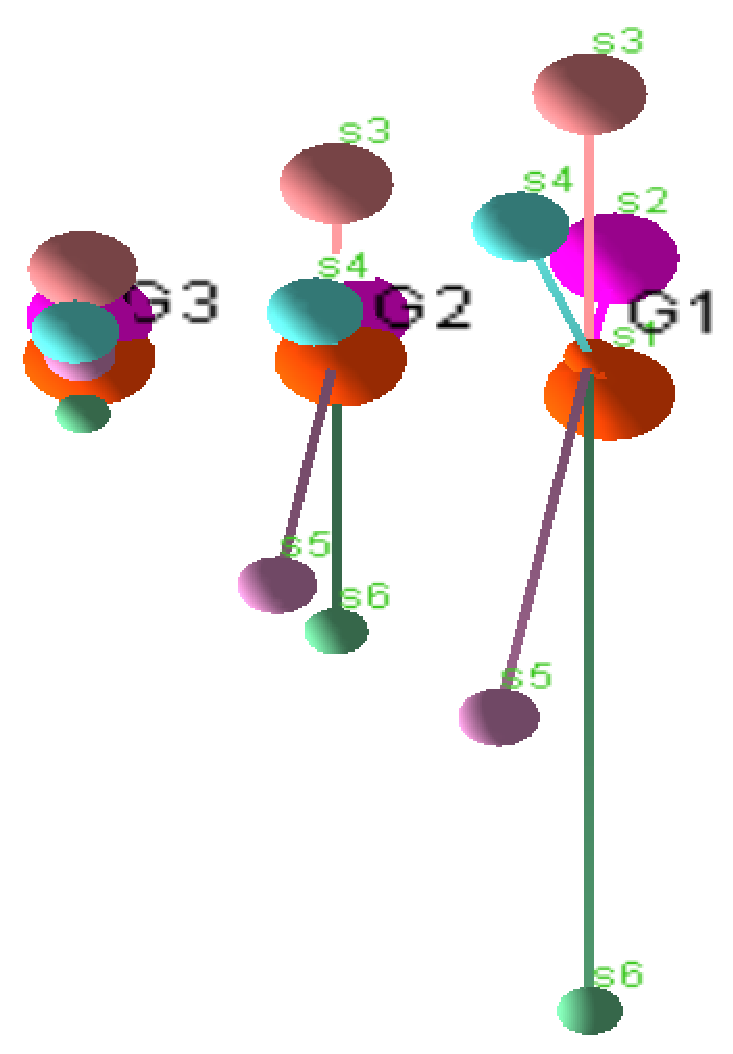
\includegraphics[width=0.4\textwidth, keepaspectratio=true]{images/angle}
\end{center}
\caption{A Star Glyph with Spheres}
\label {fig:angle}
\end{figure}

Another interaction detail is allowing the user to manipulate the scale of the plot along each axis.  This includes moving the planar star glyphs closer together for a more clustered appearance, or spreading them out more (see Figure~\ref{fig:grouped}). Grouping the data in this way visually displays where data begins to cluster across the multiple data sets. This helps analysts discover which of the outliers of the data set are more distant from the other outliers.

\begin{figure}[htb]
\begin{center}
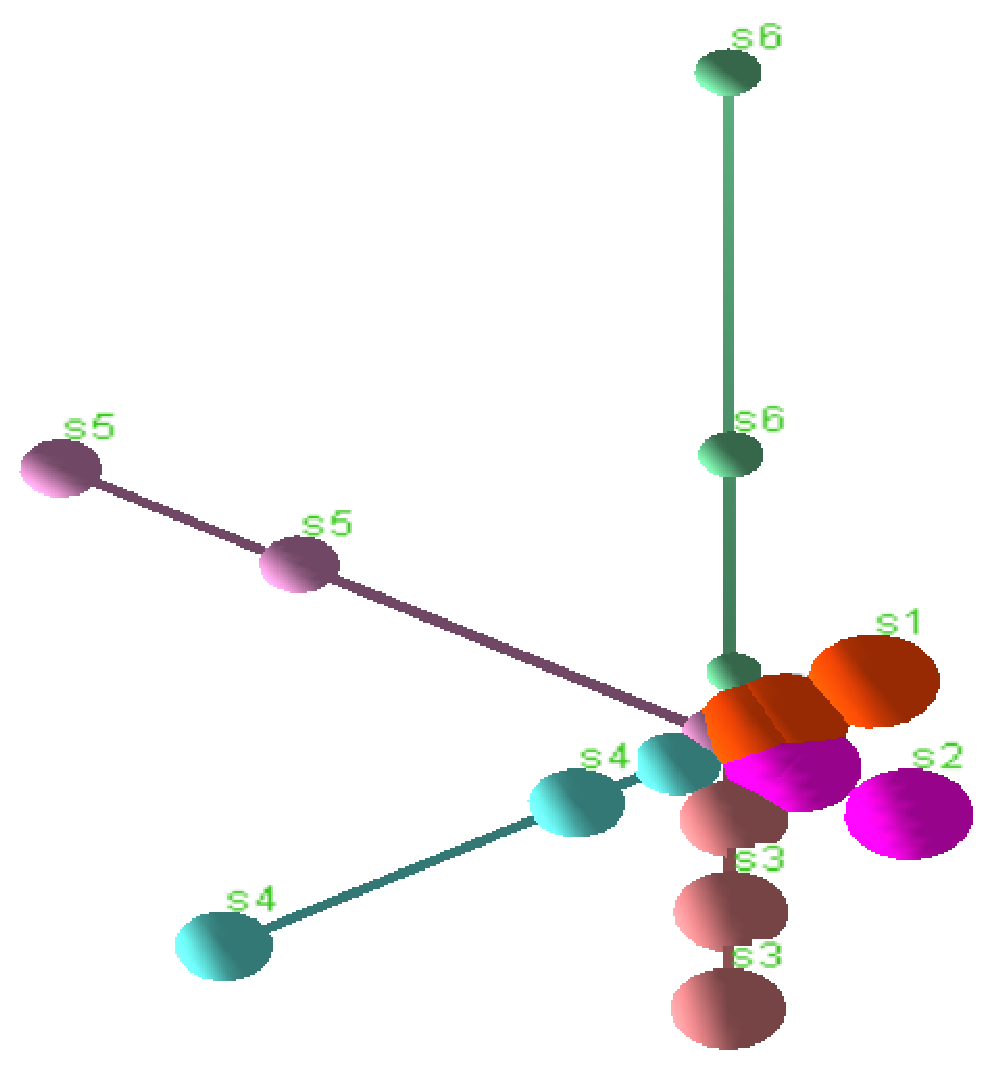
\includegraphics[width=0.4\textwidth, keepaspectratio=true]{images/grouped}
\end{center}
\caption{A Star Glyph with Spheres}
\label {fig:grouped}
\end{figure}

Another necessity is the ability to change the scales of both the spokes and the spheres.  This can make a point of interest less cluttered or easier to distinguish. 

In many visualizations, labeling of nodes can cause cluttering and are often indistinguishable from each other.  Giving the user the ability to display and hide labels of his choosing is a necessary provision.  Each spoke, sphere, and planar glyph has its own label and, often, have many more details that are too much to display in the visualization.  For instance, each sphere may be labeled with what category it represents, but the user may be interested in the exact value the size of the sphere represents.  By clicking on that particular sphere, detailed information about that category will be displayed, separate from the visualization.  Using this feature, the user can view specific details for focal points to compare and analyze.\\

We have implemented our visualization techniques in Java using JOGL, OpenGL bindings, to generate the 3D graphics. In this section we present an application of our visualization.\\


%The highest level visualization tool within TAGS is Trajectory Galaxy Visualization 3D (TrajGalaxyViz3D), a three-dimensional star glyph visualization presented in [Rusu et al., 2009a]. A star glyph is a multivariate graphing technique in which each variable represents a ray, each of which extend from a common origin with a sphere attached to the end. The length of each ray and diameter of its sphere can be used for the comparison of two attributes, where length and diameter are proportional to the value of the attribute. Traditional star glyphs are two dimensional, but TrajGalaxyViz3D displays glyphs in three dimensions, utilizing an interactive camera system to allow the user to manipulate the view. The animation of an interactive environment allows the user to maintain their orientation within the visualization and results in a more intuitive understanding of the relationship of the data by allowing it to be viewed from multiple angles than would be possible from static images. Leveraging the third dimension to display multiple glyphs at once allows for the simultaneous analysis of multiple data sets, which in turn allows more data to be presented in a single graph without overwhelming the visualization. TrajGalaxyViz3D also employs a clustering technique to more easily handle large data sets, the clustering algorithm can automatically cluster data based on its relation to the average value of all data. Clustering reduces the visibility of data close to the average while increasing visibility of outliers. When combined these techniques provide an excellent visualization of multiple large data sets for comparison by many variable groups. This capability provides a high level visualization for trajectory accuracy evaluations, where the individual data sets could, for example, represent different TPs or simulation models as in the case studies presented later in this paper.

\subsection{Trajectory Galaxy Visualization}
\label{trajGalaxyVis2d}
The Trajectory Galaxy Visualization (TrajGalaxyViz) application was developed to expand upon the capabilities of TrajGUI, providing a method for the rapid and clear visual representation of the trajectory predictions for multiple flights across one or two sets of error data simultaneously. The data generated from a scenario is grouped into clusters that represent one or more factors of the trajectory. Many flights could potentially be grouped together in this fashion. This will complement TrajGUI, allowing for evaluation of the data that will aid analysts in recognizing trends in trajectory error predictions as well as their significance. 

TrajGalaxyViz is implemented in the Java language with web start and makes extensive use of its JDBC API to access the databases containing actual flight data, predicted flight trajectories and the metrics that were discovered from the comparison of the two.   The JOGL API with its powerful graphic capabilities is used to visually represent the data. This enables TrajGalaxyViz to be launched from the web from virtually any computer with the java runtime environment, regardless of operating system and with no need for any preinstalled software.
	
\subsection{Selection Screen}
\label{selectionScreen}
The selection screen is the first screen displayed when the system is launched, see Figure 1. Here the analyst selects specifically what data is to be used and how it will be plotted.  The first option is to choose a database from a drop down list to parse for the desired flight information. The analyst must then choose an Air Route Traffic Control Center (ARTCC) from another drop-down list. In Figure 1 the analyst has chosen the faasegv1 database, ZDC which is the Washington DC ARTCC and the ROWANV7 scenario which is the ERAM trajectory predictor.  


Figure 1 – Selection Screen

 The database is then parsed to populate the drop-down list for scenarios available within the ARTCC chosen. In the example in Figure 1, the analyst has selected the ROWANV7 scenario. 

\subsection{Groupings}
\label{groupings}
The groupings list determines how the data is grouped into stars. For example if Engine Type is selected then each star will represent all the flights of a particular engine type, i.e. aircraft with jets will be plotted separately from those with piston engines. Multiple groupings can be selected in which case there will be a star for each combination of groupings. Available groupings include AC Equipage, Flight-By-Flight, Average Ground Speed, Engine Type, Flight Type, Look Ahead Time, Max Reported Altitude and End Time.

\subsection{Errors}
\label{errors}
Errors are graphed on the X and Y axis and therefore a maximum of 2 errors can be represented. Error types include horizontal, vertical, latitudinal, longitudinal, along track, cross track, slant range, time and k-value. These errors may be calculated according to various statistics including the mean, first quartile, median, third quartile, inner quartile range, minimum, maximum, range, variance, standard deviation and mean square root. In Figure 1 the mean of the horizontal and mean of the vertical error have been selected and will be displayed on the X and Y axes, respectively. 

After the selections are complete, the analyst can use the button “Continue!” to launch the next screen.  There is also the option to “Abort” which will cancel the system, or “Load” which will load a previously saved session.

\subsection{Advanced Filtering Screen}
\label{advancedFilteringScreen}
Due to the vast amount of data available an advanced filtering screen has been implemented as the metrics databases are so large that the amount of available RAM could be insufficient for some of the queries.  This screen allows the analyst to exclude data that is not pertinent to their current session which allows for easier analysis after the plot is created. Figure 2a and 2b show the Advanced Filtering window, the bar at the bottom of the screen shows the percentage of RAM that the system is using with the current choices.  As the analyst includes or excludes data the bar will adjust accordingly automatically if the “Auto-Calculate” button is checked.  The analyst may choose to uncheck the button and calculate manually by pressing the “Calculate” button. The screen divides the data in to nominal and quantitative data.

\subsection{Nominal}
\label{nominal}
Nominal data has specific categories and the analyst can choose to eliminate one or more of these categories for one or more types of data, they include the ACID CID, look ahead time, phase horizontal, phase vertical and adherence flag.

Figure 2a shows the screen with the “Nominal” tab displayed.



Figure 2a – Advanced Filtering – Nominal Tab


\subsection{Quantitative}
\label{quantitative}
Also provided is the functionality to sort by quantitative data which do not have specific categories. The included ranges are represented on the screen in Figure 2b by the sliding bar. Quantitative data may be sorted by trajectory build time, heading, time and/or ground speed.



Figure 2b – Advanced Filtering – Quantitative Tab


\subsection{Galaxy Plot}
\label{galaxyPlot}
When selecting for two errors the data is graphed as a bubble plot, or “Galaxy Plot” (see Figure 3), with errors displayed on each axis and the size of each data point proportional to the amount of data collected. TrajGalaxyViz represents the data as “stars” where each star is a cluster of data based upon the grouping factors chosen in the selection screen.

“Engine-Type” and “Look Ahead Time” were the chosen grouping factors in the example in Figure 3, so each star will represent a different engine type and look ahead time. The X-axis is the first statistic-error chosen, mean of the horizontal error, and the Y-axis is the second statistic-error chosen, mean of the vertical error. From this plot the analyst is quickly able to determine the accuracy of the data as the stars that are clustered together contain comparable accuracy measurements with those closest to the origin (0, 0) being the most accurate. The stars that are set apart on the graph show a deviation in the data, the significance of which can be quickly determined by the radius. The location of each star on the plot is therefore significant in representing how accurate the cluster of metrics data is. Stars that gather together will have similar accuracy measurements while outliers indicate deviations.
horizontal error
vertical error
number of measurements

Figure 3 – Galaxy Plot


\subsection{Histogram}
\label{histogram}
When plotting data against a single error a standard histogram (Figure 4) is used where the error is represented on the y-axis and the stars are represented as individual bars on the x-axis. By default the bars are sorted according to amount of data collected, with the bars on the left containing the most data points and the bars on the right the fewest, allowing the analyst to easily determine the significance of any given bar in relation to the rest of the data.


Figure 4 - Histogram


\subsection{Compare Plots}
\label{comparePlots}
TrajGalaxyViz implements a method of comparing two plots by creating new plot that contains every data point the original two plots have in common and using their difference as the error measurement.

\subsection{Plot Features}
\label{plotFeatures}
TrajGalaxyViz employs a wide range of features that are intended to aid the analyst in their ability to visually process the data. These features are discussed in brief as follows:

\subsection{Space Bar}
\label{spaceBar}
The “Space Bar”, as shown in Figure 5, is the main window of TrajGalaxyViz from which all functionality is contained.

Figure 5 – Space Bar

\subsection{Star Chart}
\label{starChart}
A more detailed glimpse of each “Star” is possible by clicking on it.  A “Star Chart” is displayed that contains specific information such as “Bin Name” which is the categories from the groupings, diameter, and the exact points on the X and Y axes.  Figure 6 shows the “Star Chart” for a “Star” from the Galaxy Plot in Figure 3.  The information in this “Star” has data from flights that were “Engine Type J” (Jet Engines) which had a “Look Ahead Time” of 60.   The diameter of this “Star” was 111702 and the exact location is (1.469671, 89.012403).




Figure 6 – Star Chart

\subsection{Color}
\label{color}
Plots can display an additional dimension via the color of the stars in a Galaxy Plot, or bars in a Histogram.

\subsection{Stretch Axis}
\label{stretchAxis}
TrajGalaxyViz provides the option to resize the axes through either a continuous adjustment via dragging along the axes or by right clicking the plot and selecting “set axis range” which will bring up a dialog allowing the analyst to specify a discrete range for each axis.

\subsection{Move/re-center}
\label{moveRecenter}
By choosing the move option the analyst can click anywhere on the plot and drag the mouse to re-center the plot.

\subsection{Expand-a-star}
\label{expandAStar}
TrajGalaxyViz employs a method of “expanding” stars. This option creates a Flight-by-Flight view of a new plot using the same parameters as the original plot and populates the graph with only flights contained within the selected star and then groups the data by individual flight. If a star is then expanded while in Flight-by-Flight view it opens that flight in TrajGUI for closer inspection.

\subsection{Launch TrajGUI}
\label{launchTrajGUI}
A star in a flight-by-flight plot cannot be expanded in TrajGalaxyViz any further because each star represents a single flight. Therefore this action results in TrajGUI being opened with the preselected database, ARTCC, scenario and flight fields.

\subsection{Display/hide stars}
\label{displayHideStars}
The ability to selectively hide and display stars allows the analyst to further customize their viewing options to allow for data to be pictured in the most optimal configuration. This is useful with large data sets where there are many overlapping stars that may be obscuring other data points.

\subsection{Flight-by-flight}
\label{flightByFlight}
A flight-by-flight plot is a special case of the normal plot types where each star is an individual flight.
%Once a single data set has been identified as a candidate for further analysis it can be exported to another tool in the suite, Trajectory Galaxy Visualization (TrajGalaxyViz) [Santiago et al., 2009]. TrajGalaxyViz uses weighted scatter plots, also known as bubble plots, for displaying many flights across one or two sets of error data with the option to group these flights by several factors (e.g. engine type or altitude levels). The data points are weighted by size and color which provide additional dimensions for displaying information. Data points are representative of individual flights which may optionally be grouped by some factor(s) such as aircraft type or equipage. Alternatively, flights may be grouped with a flight-by-flight factor which results in each data representing an individual flight. TrajGalaxyViz provides several additional visualization techniques such as a method for comparing plots to determine relative outliers, an expansion of any plot into a flight-by-flight view and exporting flights to another TAGS application for more detailed analysis. The “Comparison Plot” feature takes two plots, calculates the difference of each of their data points and plots them in a new window. This new Comparison Plot provides a mechanism for discovering which factors have changed the most from one data set to another. Expanding an arbitrary data point will create a new plot with each flight in that group represented as an individual data point. To determine the cause of outlying groups, individual flights can be targeted for further analysis. This expansion feature is a key step in that process as it provides access to the individual flights that compose a group, and the ability to easily identify outlying flights. Expanding a data point in a flight-by-flight plot will open that flight in TrajGUI, a convenient method for exporting outliers for more detailed analysis.

\subsection{Trajectory Graphical User Interface}
\label{trajGUI}
In 2005, the SEGV developed an upgraded version of the TrajectoryGUI for CPAT initially as part of a senior class project and continued developed through a funded internship by the FAA and a selected Rowan student. Like the prototype version developed 2001, the upgraded TrajectoryGUI is written in Java and interacts with an Oracle relational database using the Java Database Connectivity (JDBC) Application Program Interface (API) iii to execute the database queries for collecting flight data and Presented at 50th Annual Air Traffic Control Conference, October 31, 2005 flight trajectories. For this upgrade, the SEGV completely redesigned the application to use the JOGL iv library, which implements the OpenGL graphics standard v, to provide the plots.

When an analyst launches Trajectory GUI the application presents a selection window, and example of which is presented in Figure 1. The analyst uses this window to select the specific data to be used for plots and tabular display during the session.

Figure 1: Selection Window

The analyst first identifies the database that contains the tables providing the desired data for this session. These databases are the databases used by CPAT to calculate trajectory accuracy measurements [6]. The available database mappings are identified and selected from a drop-down list that is maintained in a configuration file that can be edited by the analyst. The analyst then selects the appropriate Air Route Traffic Control Center (ARTCC) from another drop-down list. In the example shown in Figure 1, the analyst has identified the local database and has selected ZME, which is the identifier for the Memphis ARTCC.

TrajectoryGUI uses the database and ARTCC information to query the database and fill the Scenario list area, which will identify the available scenario cases. In the example, two scenarios were identified and the analyst has selected the scenario case identified as ZMESAMPLE. This selection causes the Flight list area to be filled, identifying the available flights. In the example, the analyst has selected flight AIR100\_351, which represents a flight with the aircraft identification (ACID) of AIR100 and a computer identification (CID) of 351. This selection causes the Trajectory text area to be populated with the build times of the trajectories that were generated by the DST. The analyst now selects the desired trajectory to be plotted. In the example, the analyst has selected the trajectory with a build time of 40389. At this point the analyst can use the radio buttons to select the plotting option: trajectory and flight path, trajectory only, or flight only. After the desired option has been chosen, the analyst then clicks the plot button.

TrajectoryGUI queries the database and presents the application’s main window, which contains an X-Y plot, a T-Z plot, and the Metrics table for the selected flight. This window also provides the main interface with the analyst. An example of this main window is presented in Figure 2. The X-Y plot, located on the left side of the window, Presented at 50th Annual Air Traffic Control Conference, October 31, 2005 presents the positional data for the flight in a horizontal plane. It is a uniform scaled graph with units in nautical miles (nm). The positive X-axis represents east and the positive Y-axis represents north. The T-Z plot, located on the right side, presents the altitude data for the flight. The vertical units are feet and represent altitude with 0 being sea level. The horizontal units are seconds with the left most position of the graph denoting the beginning of the flight. The Metrics data is presented in a table located in below the two plots. The table is filled with the accuracy measurement data selected from the database. At the bottom of the main window is a text area that is used to report information such as operational results, program mode, and status, and errors. At the top of this window an array of functions are available to the analyst that can be used to probe the plots.

Figure 2: Main TrajectoryGUI Window

The analyst can manipulate the X-Y plot by using the Re-center, Zoom In, Zoom Out, Offset Trajectory, Move Legend, and Reset functions. For example, in Figure 2, the position data for the flight is shown in a viewing area of 10,000 square nautical miles. The analyst can re-center the plot by positioning the mouse at any position on the plot and clicking the left mouse button. The plot will be redrawn with the clicked position becoming the center of the plot viewing area. Figure 3 shows the result of re-centering to the area around the beginning of the flight data and zooming in to a plot view area of 100 square nautical miles. The offset functionality is useful if the trajectory lies near or directly on top of the flight’s actual path. If this is the case, the analyst can offset the trajectory creating separation between the data. The analyst uses the Move Legend Presented at 50th Annual Air Traffic Control Conference, October 31, 2005 function when the legend is located in an area where data is displayed. Resetting a plot allows the analyst to return to the initial viewing area of the plot.

Other functions available to the analyst include: Get Position, Get Distance, Clear Position, Clear Distance, Clear All Positions, and Clear All Distances. When Get Position is activated, the analyst can click near any node, a position stamp will be applied to the closest node to the clicked location and that node’s precise X and Y values will display in the text area. Examples of position stamps are shown in Figure 3 at the beginning of each path. When Get Distance is activated, the analyst can click near two nodes to find the exact distance between the nodes. These two nodes are usually time- coincident points. After the two nodes have been selected, a distance line will be drawn connecting the two nodes and the exact distance will be computed and displayed in the text area. When clearing positions and distances the analyst simply clicks near the item and the item is removed. Clearing all functionalities removes all of the particular items selected.

Figure 3: Manipulated X-Y Plot

Another important feature in the X-Y plot is the labeling of time tags, which allow the analyst to visualize the accuracy of a trajectory prediction at a specific time. The time tags are applied starting at some time point that is common in the track data and trajectory data. The time tags are based on two features: time tag frequency f, which is an integer value representing one time tag per f nodes, and offset o, which is an integer value representing o nodes from the first common time point. The analyst is given the capability to vary both the frequency and the offset value. In addition, time tags can be applied one at a time using the Get Time Tag function. These types of time tags are Presented at 50th Annual Air Traffic Control Conference, October 31, 2005 referred to as manually applied time tags and are activated when the analyst clicks on node to append time tag. Additionally, these manual time tags can be cleared similar to the position stamps and distance lines. After time tags have been applied, the time tags may overwrite viewing areas in the plot. As a result, the ability to rotate time tags is also given to the analyst.

The T-Z plot window displays the T and Z coordinates of the flight’s track data and the flight’s trajectory data in an interactive coordinate system. Many of the same features exist for the T-Z plot, but they are used independently within the plots. Within the T-Z plot, the analyst can Re-center, Zoom In, Zoom Out, Offset Trajectory, and Reset. In addition, the analyst can use the functions Get Position, Clear Position, and Clear All Positions. Like the X-Y plot, the legend can conceal valuable information at times, while the analyst can take advantage of the Move Legend function.

Additional capabilities of TrajectoryGUI include:
an image export of the X-Y and T-Z plots for the use in presentations and reports
a file export of the Metrics data in a comma delimited file for import into other application programs
an interface that provides the ability to select and deselect the metrics that will be displayed in the Metrics table
a configuration file for maintaining lists of:
-accessible databases along with their connection parameters
-the default metric fields to be included in the Metrics table
-the desired colors for display of the actual flight path and of the trajectory path

%The lowest level tool in the suite is Trajectory Graphical User Interface (TrajGUI) which focuses on the visualization of a small number of flights in detail [Santiago et al., 2005]. Since its original design and development, TrajGUI has gone through numerous iterations of enhancements via the FAA and Rowan collaboration. TrajGUI provides a rapid and clear visual representation of trajectory predictions via a two dimensional plot, where the dimensions may be representative of error or positional data. Positional dimensions are those which comprise a trajectory (i.e. latitude, longitude, altitude and time) while error data is based on metrics generated for each flight. These plots serve as a means of comparing one or many predicted trajectories to the actual ground truth of a flight (as flown). Plots may contain multiple flight paths and each flight path may have many trajectories associated with them that were calculated at different times during the flight. For example, plotting a flight by latitude and longitude values will create a plot representative of a “top down” view. Another common method is plotting by altitude and time which results in an altitude profile of the flight over time. These different views allow for easy comparison of the accuracy of the trajectories to the actual flight path and to each other by virtually any variable of interest. TrajGUI is intended to be a micro-scale analysis tool, providing researchers the ability to peer deeply into the details of select flights of interest and the trajectories the TP generated. 

\section{Statistics}
\label{statisitics}

\subsection{Metrics}
\label{metrics}

The first step in the comparison of trajectory modeling tools is to determine what statistics they will be evaluated against. The S\&A Team has developed a set of metrics to measure TP accuracy using the difference between predicted and future path of the aircraft, and from these metrics we have chosen to evaluate based on the mean horizontal and vertical error [Paglione et al., 2007]. This provides a quantifiable method of assessment for trajectory predictors which are then, optionally, grouped by certain factors for evaluation.

\subsection{Factors}
\label{factors}
The following grouping factors have been chosen:
Engine Type – Jet, Turbo Prop or Piston
Maximum Altitude – Range from 0 to 46000 feet, divided into six equal bins
Vertical Phase of Flight – Ascending, level or descending

For each of these three factors, flights will additionally be grouped by look-ahead-time for the TP analysis (not applicable for simulation). Look-ahead-time is how far into the future the TP is generating trajectories for. Intuitively it is more difficult to accurately predict trajectories for longer look-ahead-times (e.g. it is easier to say where a flight will be in ten seconds than ten minutes).

Vertical phase of flight was chosen as a factor because it was specifically noted in a technical note on the 2007 ERAM FAT/RFR as a challenging factor for DSTs. Another factor that greatly affects TP accuracy is engine type. Due to the nature of the aircraft that different engine types are used for, TP accuracy may fluctuate widely from one engine type to another. Jet engines, for example, are used primarily by large commercial aircraft which have relatively little deviation in their flight plans. On the other hand, piston engines tend to be used for smaller, often personal, aircraft and because they are more maneuverable they are harder for a TP to accurately predict. As vertical phase and engine type both have discrete values, we have decided to select a third factor which is continuous. Maximum altitude is a good candidate because it fills this requirement and provides another vertical factor for comparison.

%\section{Methodologies}
%\label{methodologies}

\section{Case Study \#1 - Maximum Altitude, ERAM-FAT vs ERAM-Corrective Action}
\label{caseStudy1}

An important component of TP testing and evaluation is the general refinement and improvement of subsequent releases, and ensuring that there are no areas of declining performance compared to earlier versions. In this case we will be looking at data from two versions of ERAM, one using the data from the FAT and a second from the corrective action process of addressing PRs. Moreover, a transition from a macroscopic TP-wide analysis into a flight-by-flight trajectory prediction accuracy investigation will be presented. The validation process involves both acceptance testing, which evaluates the current version based on the requirements, and regression testing, which ensures that each new iteration is performing at least as well as the legacy system.

Of the three factors chosen for analysis (maximum altitude, engine type and vertical phase of flight), maximum altitude produced the most interesting data and will be the focus of our first case study. Altitude has already been mentioned as an important factor in evaluating TP performance because of the difficulty inherent in predicting it accurately; therefore we have grouped the flight data by maximum altitude and look-ahead-time to see its impact on trajectory accuracy.


Figure 1 – ERAM-FAT vs. ERAM-Corrective Action

Figure 1 shows the graphs of ERAM-FAT and ERAM-Corrective Action grouped by maximum altitude and look-ahead-time. It would be difficult to discern what, if any, are the significant differences between these plots without more detailed analysis. A comparison plot, presented in Figure 2, is the ideal method of visualizing the differences between two sets of data.
 

Figure 2 – Comparison Plot between ERAM-FAT and ERAM-Corrective Action

Comparison plots chart the mathematical difference between two data sets, so the four outliers circled in Figure 2 are indicative of a substantial improvement in the vertical accuracy of ERAM’s TP from one version to the next. Further examination reveals the outliers represent flights in the highest altitude bin across all look-ahead-times, i.e. they are all the flights in the 42,000-46,000ft range. This means that the TP was able to generate trajectories for flights in the highest maximum altitude bin (42,000-46,000) much more accurately compared to the other maximum altitude bins. This improvement to the trajectory prediction capability of ERAM demonstrates this was likely a targeted area for development. These are indicators of an aspect that warrants further investigation and analysis, the next step is to identify individual flights of interest which can then be examined in greater detail in TrajGUI.


Figure 3 – ERAM-FAT outlier in TrajGalaxyViz (left) and TrajGUI (right)


Figure 4 – ERAM-Corrective Action outlier in TrajGalaxyViz (left) and TrajGUI (right)

Creating a flight-by-flight plot of the flights in the 42,000-46,000ft range reveals a single outlier in both ERAM-FAT and ERAM-Corrective Action. The outlier for both TPs has the same aircraft identification (call sign) which indicates it is the same flight. Examining this flight in greater detail may be useful in determining both the reason for the inaccuracy in ERAM-FAT and why it was not corrected for ERAM-Corrective Action. Figures 3 and 4 show a flight-by-flight TrajGalaxyViz plot and a corresponding single flight TrajGUI plot side by side. The TrajGUI plots have been created from the outlying flight that is circled in red in the TrajGalaxyViz plot. The TrajGUI plots show the track of the aircraft in red and trajectories in miscellaneous other colors. The TrajGUI plots for both ERAM-FAT and ERAM-Corrective Action appear to indicate that the reason for error of the outlier flight was that the track passed over an airport, but the trajectories were generated for a departure.

From this analysis we have learned that there was likely a concerted effort to improve the accuracy of ERAM’s TP at peak altitudes and that there may be an issue causing trajectories to be incorrectly generated for flights flying over airports that is present in both versions of ERAM. This demonstrates the ability of these tools in finding both the strengths and weaknesses in dataset. The strengths provide a measure of progress from one version to the next while the weaknesses determine how much work remains. 

\subsection{Discussion of other factors}
\label{otherFactors}
While maximum altitude was found to be the most interesting factor for analysis, vertical phase and engine type may still yield important results.

\subsection{Vertical Phase of Flight}
\label{verticalPhase}
The first of the failed RFR accuracy requirements was vertical trajectory accuracy for both level and transitioning flight. For transitioning flights, descent, in particular, is a challenging area and was noted in the conclusion of the 2007 ERAM FAT/RFR technical note. The process of investigating descent may involve narrowing the search to specific areas such as top of descent, descending to avoiding poor flight conditions (traffic, weather, turbulence, etc), involuntary descent (loss of power or lift, downdraft, etc), to enter warmer air, or to take advantage of wind direction of a different altitude. For example, top of descent is the point at which an aircraft transitions from the level cruise phase to its descent into final approach, and through the examination of outliers that match a top of descent profile we may discover some significant improvement in this aspect of trajectory data from ERAM-FAT to ERAM-Corrective Action.

\subsection{Engine Type}
\label{engineType}
The focus of analysis so far has been limited to vertical error, however when looking at engine type there is a large difference in the horizontal error of aircrafts with piston engines. This difference amounts to an average improvement on the order of nearly two nautical miles, which is significant. A possible contribution to the error in ERAM-FAT, and in turn the improvement in ERAM-Corrective Action, is from flights being diverted off their inteneded routes without their track being updated. This leads the TP to continually generate trajectories back to the original route resulting in a large degree of horizontal error. The issue of vectoring of routes was found to be the cause of error for some flights so it is possible that this problem was addressed in ERAM-Corrective Action and is the cause of overall improvement in horizontal error for piston aircraft.

\section{Case Study \#2 – Simulation Models}
\label{caseStudy2}
This case study will focus on the horizontal error of the four developmental trajectory predictor models (non-operational). As mentioned before, these TPs were developed in-house by the S\&A Team to support simulation and modeling activities and used in the research of future NextGen concepts. Furthermore, this case study will transition between a three staged TP accuracy analytical process; beginning at a macroscopic TP system effect, and diving into a microscopic flight specific example. It is expected that the performance of the predictors, ordered best to worst, will be BADA, followed by Hybrid Merge, then Flight Plan and finally Linear Predictor. A single star glyph of the BADA TP is presented in Figure 5 with color coded factors; green spokes are vertical phases, red are engine types and blue are maximum altitude bins. Mean horizontal error is represented by distance from origin while sphere diameter indicates weight.

 
Figure 5 – TrajGalaxyViz3D Single data set (side and front view)

Figure 6 and 7 show how multiple data sets are displayed in TrajGalaxyViz3D. The front view is a particularly important component of the visualization as it provides an effective means of overlaying multiple data sets. A cursory look at the glyphs confirms our expectations of relative TP performance.


Figure 6 – TrajGalaxyViz3D Four data sets (side view)


Figure 7 – TrajGalaxyViz3D Four data sets (front view)

Closer analysis reveals that the BADA TP’ss performance for ascending flights is slightly worse than Hybrid Merge, investigating this discrepancy by plotting BADA and Hybrid Merge in TrajGalaxyViz yield the graphs in Figure 8. These graphs are plotted by latitudinal and longitudinal error (the components of horizontal error) and grouped by look-ahead-times 0, 300, 600 and 900 seconds. Although Hybrid Merge has slightly less horizontal error overall, BADA has much better performance at look-ahead-time 900s (15 minutes).


Figure 8 – BADA (left) and Hybrid Merge (right) in TrajGalaxy Viz

In order to determine the cause for this inconsistency the bin for look-ahead-time 900s may be expanded into a flight-by-flight plot to examine individual flights. Comparing the flight-by-flight plots reveals the flights with the highest difference in error (i.e. greatest improvement from Hybrid Merge to BADA), of which one was selected for further analysis. Figure 9 shows the same flight for BADA and Hybrid Merge opened in TrajGUI. Determining the cause of error variance for this flight may give insight into the variance of the error for both TPs as a whole.


Figure 9 – BADA Adjusted Trajectory (left) vs Hybrid Merge (right)

One reason for improvement appears to be due to a change in the heading of a BADA predicted trajectory. The reason for this change is a result of BADA TP’s ability to alter trajectory speed because it is using a better aircraft performance model whereas Hybrid Merge must maintain cruise speed. In this case the speed of the predicted trajectory was decreased which caused it to overrun the Hybrid Merge trajectory, a fairly common problem which results in the trajectory heading being set to the destination airport. In this situation the change of heading decreased overall horizontal error and it is possible that the relatively long look-ahead-time of 900s magnified the difference significantly. 

If there is more sensitivtydue to longer look ahead times then this could explain why the BADA TP performs better at look-ahead-time 900s, but worse overall. The first case study revealed that these tools can be used to find the strengths and weaknesses of a trajectory predictor, and from the second we have discovered they are also useful for finding inconsistencies in the data and providing possible explanations. These valuable insights are the benefit that visualization tools provide to testing and evaluation processes as without some method of visualizing the data this type of finding could easily be missed by analysts.
 
\section{Conclusion}
\label{conclusion}
These case studies serve to outline a process for the analysis of aircraft trajectory prediction data using a suite of data visualization tools. This process involves a staged approach starting with a high level view and then filtering down to examine specific points of interest in more detail at a lower level. This is both an intuitive and effective means for analysts to evaluate TPs and determine specific areas of strength and, more importantly, weakness. The tools used in these studies were developed by the SEGV group at Rowan University and represent a larger effort on part of the FAA to develop a testing and evaluation infrastructure in support of the development and implementation of NextGen. Trajectory-based operations are identified in the NextGen Concept of Operations as a key capability required to ensure the success of NextGen [Romanelli et al., 2009]; thus, it is essential that the accuracy of trajectory prediction software be tested and validated.

\begin{comment}
\section{Acronyms}
\label{acronyms}
BADA – Base of Aircraft Data
CPAT – Conflict Probe Assessment Team
CTAS – Center TRACON Automation System
DST – Decision Support Tool
ERAM – En Route Automation Modernization
FAA – Federal Aviation Administration
FAT – Factory Acceptance Test
HCS – Host Computer System
PR – Problem Report
TAGS – Trajectory Analysis Graphical Suite
TP – Trajectory Predictor
TBO – Trajectory Based Operations
URET – User Request Evaluation Tool
RFR – Run For Record
\end{comment}
\end{document}
